\documentclass{assignment}
\UsingEnglish
\ProjectInfos*{Intro to Communication System}{EE140}{Fall, 2020}{Assignment 5}{Due time : 10:15, Oct 23, 2020 (Friday)}{陈稼霖}{45875852}
\begin{document}
\begin{prob}[Definition of FM, 10pts]
    An FM modulator has output $x_c(t)=10\cos[2\pi f_ct+2\pi f_d\int_0^tm(\tau)\,\mathrm{d}\tau]$, where $f_d=20$ Hz/Volt. Assume that $m(t)=3\Lambda\left(\frac{1}{3}(t-3)\right)$, as shown in Figure \ref{A-5-P-1}.
    \begin{figure}[h]
        \centering
        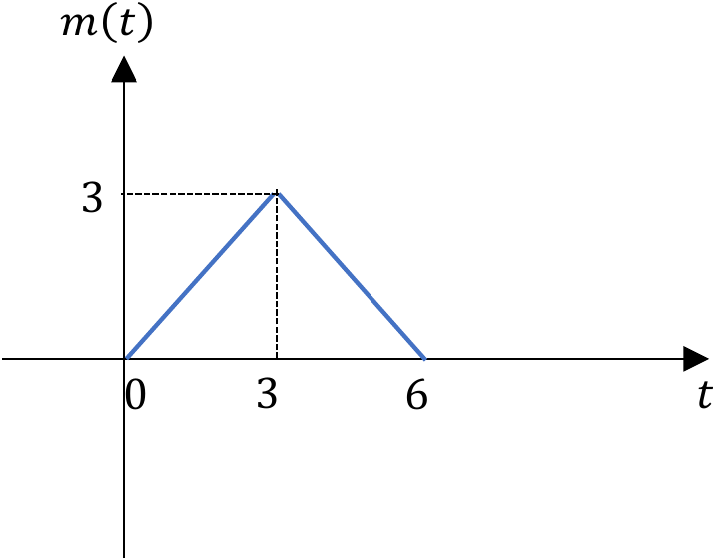
\includegraphics[width=.5\columnwidth]{Assignment-5-Problem-1.png}
        \caption{}
        \label{A-5-P-1}
    \end{figure}
    \begin{itemize}
        \item[1)] Determine the phase deviation in radians.
        \item[2)] Determine the frequency deviation in hertz.
        \item[3)] Determine the peak frequency deviation in hertz.
        \item[4)] Determine the peak phase deviation in radians.
    \end{itemize}
\end{prob}
\begin{sol}
    \begin{itemize}
        \item[1)] The phase deviation in radians is
        \begin{align}
            \phi(t)=&2\pi f_d\int_0^tm(\tau)\,\mathrm{d}\tau=40\pi\int_0^t3\Lambda\left(\frac{1}{3}(\tau-3)\right)\,\mathrm{d}\tau=\left\{\begin{array}{ll}
                60\pi t^2,&0\leq t\leq 3,\\
                -60\pi t^2+720\pi t-1080\pi,&3<t\leq 6,\\
                1080\pi,&t>6.
            \end{array}\right.\quad(\text{unit: rad})
        \end{align}
        \item[2)] The frequency deviation in hertz is
        \begin{align}
            \frac{1}{2\pi}\frac{\mathrm{d}\phi}{\mathrm{d}t}=&\frac{1}{2\pi}\frac{\mathrm{d}\left[2\pi f_d\int_0^tm(\tau)\,d\tau\right]}{\mathrm{d}t}=f_dm(t)=60\Lambda\left(\frac{1}{3}(t-3)\right)\quad(\text{unit: Hz}).
        \end{align}
        \item[3)] The peak frequency deviation in hertz is
        \begin{align}
            \Delta f=\max\left[\abs{\frac{1}{2\pi}\frac{\mathrm{d}\phi}{\mathrm{d}t}}\right]=60\text{ Hz}.
        \end{align}
        \item[4)] The peak phase deviation in radians is
        \begin{align}
            \Delta\phi=\max[\abs{\phi(t)}]=1080\text{ rad}.
        \end{align}
    \end{itemize}
\end{sol}

\begin{prob}[Definition of PM, 10pts]
    A PM modulator has output $x_c(t)=10\cos[2\pi f_ct+k_pm(t)]$, where $k_p=20$ radian/Volts. Assume that $m(t)=3\Lambda\left(\frac{1}{3}(t-3)\right)$, as shown in Figure \ref{A-5-P-1}.
    \begin{itemize}
        \item[1)] Determine the phase deviation in radians.
        \item[2)] Determine the frequency deviation in hertz.
        \item[3)] Determine the peak frequency deviation in hertz.
        \item[4)] Determine the peak phase deviation in radians.
    \end{itemize}
\end{prob}
\begin{sol}
    \begin{itemize}
        \item[1)] The phase deviation in radians is
        \begin{align}
            \phi(t)=k_pm(t)=60\Lambda\left(\frac{1}{3}(t-3)\right)\text{ (unit: rad)}.
        \end{align}
        \item[2)] The frequency deviation in hertz is
        \begin{align}
            \frac{1}{2\pi}\frac{\mathrm{d}\phi}{\mathrm{d}t}=\left\{\begin{array}{ll}
                \frac{30}{\pi},&0\leq t\leq 3,\\
                -\frac{30}{\pi},&3< t\leq 6,\\
                0,&t>6.
            \end{array}\right.(\text{unit: Hz})
        \end{align}
        \item[3)] The peak frequency deviation in hertz is
        \begin{align}
            \Delta f=\max\left[\abs{\frac{1}{2\pi}\frac{\mathrm{d}\phi}{\mathrm{d}t}}\right]=\frac{30}{\pi}\text{ Hz}.
        \end{align}
        \item[4)] The peak phase deviation in radians is
        \begin{align}
            \Delta\phi=\max[\abs{\phi(t)}]=60\text{ rad}.
        \end{align}
    \end{itemize}
\end{sol}

\begin{prob}
    An FM modulator has $f_c=2000$ Hz and $f_d=20$ Hz/Volt. The modulating message signal is $m(t)=5\cos 20\pi t$.
    \begin{itemize}
        \item[1)] What's the peak frequency deviation?
        \item[2)] What's the modulation index?
        \item[3)] Is this narrow band FM? Why?
        \item[4)] If the same $m(t)$ is used for a phase modulator, what must $k_p$ be to yield the modulation index given in 1)?
        \item[5)] Determine the approximate bandwidth of the FM signal, using Carson's rule.
        \item[6)] Determine the bandwidth by transmitting only those side frequencies whose amplitude exceed $1$ percent of the unmodulated carrier amplitude. Use the Table from Page 163 for this calculation. (Hint: find $n_{\max}$, which is the largest value of the integer that satisfies the requirement $J_n(\beta)>0.01$. Then $B=2n_{\max}f_m$.)
        \item[7)] Repeat your calculation in 5), assuming that the amplitude of the modulating signal $m(t)$ is doubled. (Hint: $m(t)=10\cos 20\pi t$.)
        \item[8)] Repeat your calculation in 5), assuming that the frequency of the modulating signal $m(t)$ is doubled. (Hint: $m(t)=5\cos 40\pi t$.)
    \end{itemize}
\end{prob}
\begin{sol}
    \begin{itemize}
        \item[1)] 
        \item[2)] 
        \item[3)] 
        \item[4)] 
        \item[5)] 
        \item[6)] 
        \item[7)] 
        \item[8)] 
    \end{itemize}
\end{sol}

\begin{prob}[Bandwidth of Wideband PM, 20pts]
    Consider a PM signal produced by a sinusoidal modulating wave $m(t)=A_m\cos 2\pi f_mt$ using a modulator with a phase deviation constant equal to $k_p$ radians per volt. The unmodulated carrier wave has frequency $f_c$ and amplitude $A_c$.
    \begin{itemize}
        \item[1)] Show that if the maximum phase deviation of the PM signal is much larger than $1$ radian, the bandwidth of the PM signal varies linearly with the modulation frequency $f_m$.
        \item[2)] Compare this characteristic of a wideband PM signal with that of the corresponding wideband FM signal.
    \end{itemize}
\end{prob}
\begin{sol}
    \begin{itemize}
        \item[1)] 
        \item[2)] 
    \end{itemize}
\end{sol}

\begin{prob}[Generation of Wideband FM Signal, 20pts]
    A narrowband FM has a carrier frequency of $110$ kHz and a deviation ratio of $0.05$. The bandwidth of the modulating signal is $10$ kHz. This narrowband FM signal is used to generate a wideband FM signal with a deviation ratio of $20$ and a carrier frequency of $100$ MHz. We use the Armstrong indirect FM transmitter in Figure \ref{A-5-P-5} to accomplish this. Give the required value of frequency multiplication $n$. Also, fully define the mixer by giving two permissible frequencies for local oscillator, and define the required bandpass filter (the center frequency and the bandwidth using Carson's rule).
    \begin{figure}[h]
        \centering
        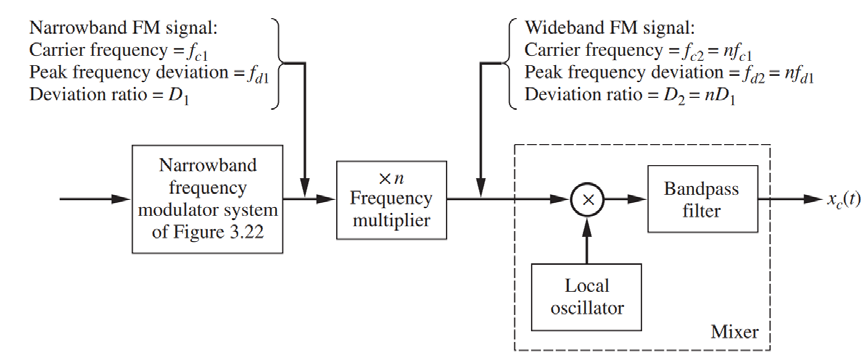
\includegraphics[width=.8\columnwidth]{Assignment-5-Problem-5.png}
        \caption{}
        \label{A-5-P-5}
    \end{figure}
\end{prob}
\begin{sol}
    
\end{sol}
\end{document}